\documentclass[11pt,a4paper]{article}

% --- packages -------------------------------------------------------------
\usepackage[utf8]{inputenc}
\usepackage[T1]{fontenc}
\usepackage{lmodern}
\usepackage{microtype}
\usepackage[a4paper,margin=2.4cm,headheight=14pt]{geometry}
\usepackage{amsmath,amssymb,mathtools}
\usepackage{graphicx}
\usepackage{booktabs}
\usepackage{tabularx}
\usepackage{array}
\usepackage{xcolor}
\usepackage{enumitem}
\usepackage{caption}
\usepackage{subcaption}
\usepackage[scaled=0.85]{beramono}
\usepackage{listings}
\usepackage{titling}
\usepackage{titlesec}
\usepackage{fancyhdr}
\usepackage[round,authoryear]{natbib}
\usepackage{hyperref}

\definecolor{accent}{HTML}{0F5C8A}
\definecolor{accent2}{HTML}{C2410C}
\definecolor{rule}{HTML}{8895A1}
\definecolor{codebg}{HTML}{F5F7FA}
\definecolor{codekw}{HTML}{0F5C8A}
\definecolor{codestr}{HTML}{067D17}
\definecolor{codecom}{HTML}{6E7781}
\definecolor{boxrule}{HTML}{B8C7D8}

% Per-clip accent colours, matched to the figures.
\definecolor{ex01}{HTML}{1F77B4}
\definecolor{ex02}{HTML}{D97706}
\definecolor{ex03}{HTML}{2E7D32}
\definecolor{ex04}{HTML}{7E3FF2}
% Family colours (raw / oscillatory / complexity).
\definecolor{famraw}{HTML}{1B6CA8}
\definecolor{famosc}{HTML}{B07005}
\definecolor{famcpl}{HTML}{6A2C7E}

\hypersetup{
  colorlinks=true,
  linkcolor=accent,
  urlcolor=accent,
  citecolor=accent,
  pdftitle={Reading sea-wave dynamics from video (HNA video module, v3)},
  pdfauthor={HumanNatureAttunement},
}

\titleformat{\section}
  {\Large\bfseries\color{accent}}
  {\thesection}{0.6em}{}
  [{\color{rule}\titlerule[0.6pt]}]
\titleformat{\subsection}
  {\large\bfseries\color{accent}}
  {\thesubsection}{0.55em}{}

\lstdefinelanguage{pythonish}{
  morekeywords={def,class,return,if,else,elif,for,while,in,not,and,or,from,import,
                as,with,True,False,None,lambda,try,except,finally,pass,raise,
                yield,is,break,continue},
  morecomment=[l]\#,
  morestring=[b]",
  morestring=[b]'
}
\lstset{
  language=pythonish,
  basicstyle=\ttfamily\small,
  keywordstyle=\color{codekw}\bfseries,
  stringstyle=\color{codestr},
  commentstyle=\color{codecom}\itshape,
  numberstyle=\tiny\color{codecom},
  numbers=left, numbersep=8pt,
  backgroundcolor=\color{codebg},
  frame=single, framesep=4pt, framerule=0pt, rulecolor=\color{codebg},
  breaklines=true, breakatwhitespace=true,
  columns=fullflexible, keepspaces=true,
  xleftmargin=10pt, xrightmargin=4pt,
  aboveskip=8pt, belowskip=8pt,
}

\pagestyle{fancy}
\fancyhf{}
\fancyhead[L]{\small\color{rule}HNA toolbox -- video module (v3)}
\fancyhead[R]{\small\color{rule}\thepage}
\renewcommand{\headrulewidth}{0pt}
\fancypagestyle{plain}{\fancyhf{}\fancyfoot[R]{\small\color{rule}\thepage}}

\setlength{\droptitle}{-1.4cm}
\title{\vspace{-1cm}\Huge\bfseries Reading sea-wave dynamics from video \\[2pt]
  \large\mdseries A multi-scale toolbox for cross-modal coupling \\[2pt]
  \large\mdseries \texttt{HNA.modalities.video}}
\author{HumanNatureAttunement project \\[-2pt]
  \small Antoine Bellemare \& Mar Estarellas}
\date{\small \today}

\newcommand{\code}[1]{\texttt{\small #1}}
\newcommand{\famraw}[1]{\textcolor{famraw}{\textbf{#1}}}
\newcommand{\famosc}[1]{\textcolor{famosc}{\textbf{#1}}}
\newcommand{\famcpl}[1]{\textcolor{famcpl}{\textbf{#1}}}

\newcommand{\keybox}[2]{%
  \par\vspace{6pt}\noindent
  {\color{boxrule}\hrule height 0.6pt}\vspace{3pt}
  \noindent\textbf{\color{accent}#1}\par\vspace{2pt}
  \noindent #2\par\vspace{3pt}
  {\color{boxrule}\hrule height 0.6pt}\vspace{6pt}\noindent\ignorespaces}

\begin{document}
\maketitle
\thispagestyle{plain}

\begin{abstract}\noindent
A wave is at once a regular oscillator and an unpredictable turbulent
surface, and human physiology -- breath, heartbeat, brain rhythms --
responds to both faces of it. To make that responsiveness measurable
the HumanNatureAttunement project needs the visual modality on the
same footing as the audio side: a battery of 1-D signals, sampled at
the frame rate, that capture what the eye is doing without losing
multi-scale structure. \code{HNA.modalities.video} delivers exactly that,
organised along two axes -- a \emph{spatial scale} of analysis
(whole-image, per-patch, per-pixel) and a \emph{feature family}
(\famraw{raw}, \famosc{oscillatory}, \famcpl{complexity}). The product
is a 3-by-3 framework, nine cells of extractors whose 1-D outputs are
drop-in inputs to the project's coupling toolbox. We illustrate every
cell with a single set of four contrasting clips and close with a
cross-clip fingerprint that visibly groups by family.
\end{abstract}

\vspace{4pt}\hrule height 0.6pt\vspace{6pt}
{\small\color{rule}
The Python sub-package \code{src/HNA/modalities/video/} is a
one-to-one mirror of the framework: each cell of
Fig.~\ref{fig:framework} maps to a file in that directory.}
\vspace{6pt}\hrule height 0.6pt
\tableofcontents
\vspace{6pt}

% =========================================================================
\section{What this module is for}\label{sec:intro}
% =========================================================================

The HumanNatureAttunement project asks whether the human body and
brain \emph{entrain} to natural rhythmic stimuli, and whether the
strength of that entrainment depends on attention or on the listener's
state. The audio-side pipeline is established: the acoustic envelope
of a wave recording is correlated with EEG band power, and the
coupling is stronger under undivided attention. The video module
extends the question symmetrically: \emph{does the brain (or the
heart, or the muscles) track the visual envelope of the same
stimulus?}

That symmetry has a cost: a wave looks like many things at once. A
breaking crest is a sharp \famcpl{edge}; the swell is a slow horizontal
\famosc{stripe} travelling across the frame; foam break-up is a
turbulent \famcpl{fractal texture}. Each has its own characteristic
timescale and its own plausible coupling target on the physiological
side. The toolbox therefore gives us a generous menu of 1-D signals,
each describing a different visual facet of the same clip.

\keybox{Design rules}{%
Every signal is \textbf{1-D, sampled at the frame rate},
\textbf{physically interpretable}, and \textbf{cheap}: minutes of HD
footage in seconds on CPU. These three rules let the same coupling
tools that already work on EEG, HRV and audio plug directly into the
visual modality.}

% =========================================================================
\section{The framework, in one figure}\label{sec:framework}
% =========================================================================

\begin{figure}[ht]
  \centering
  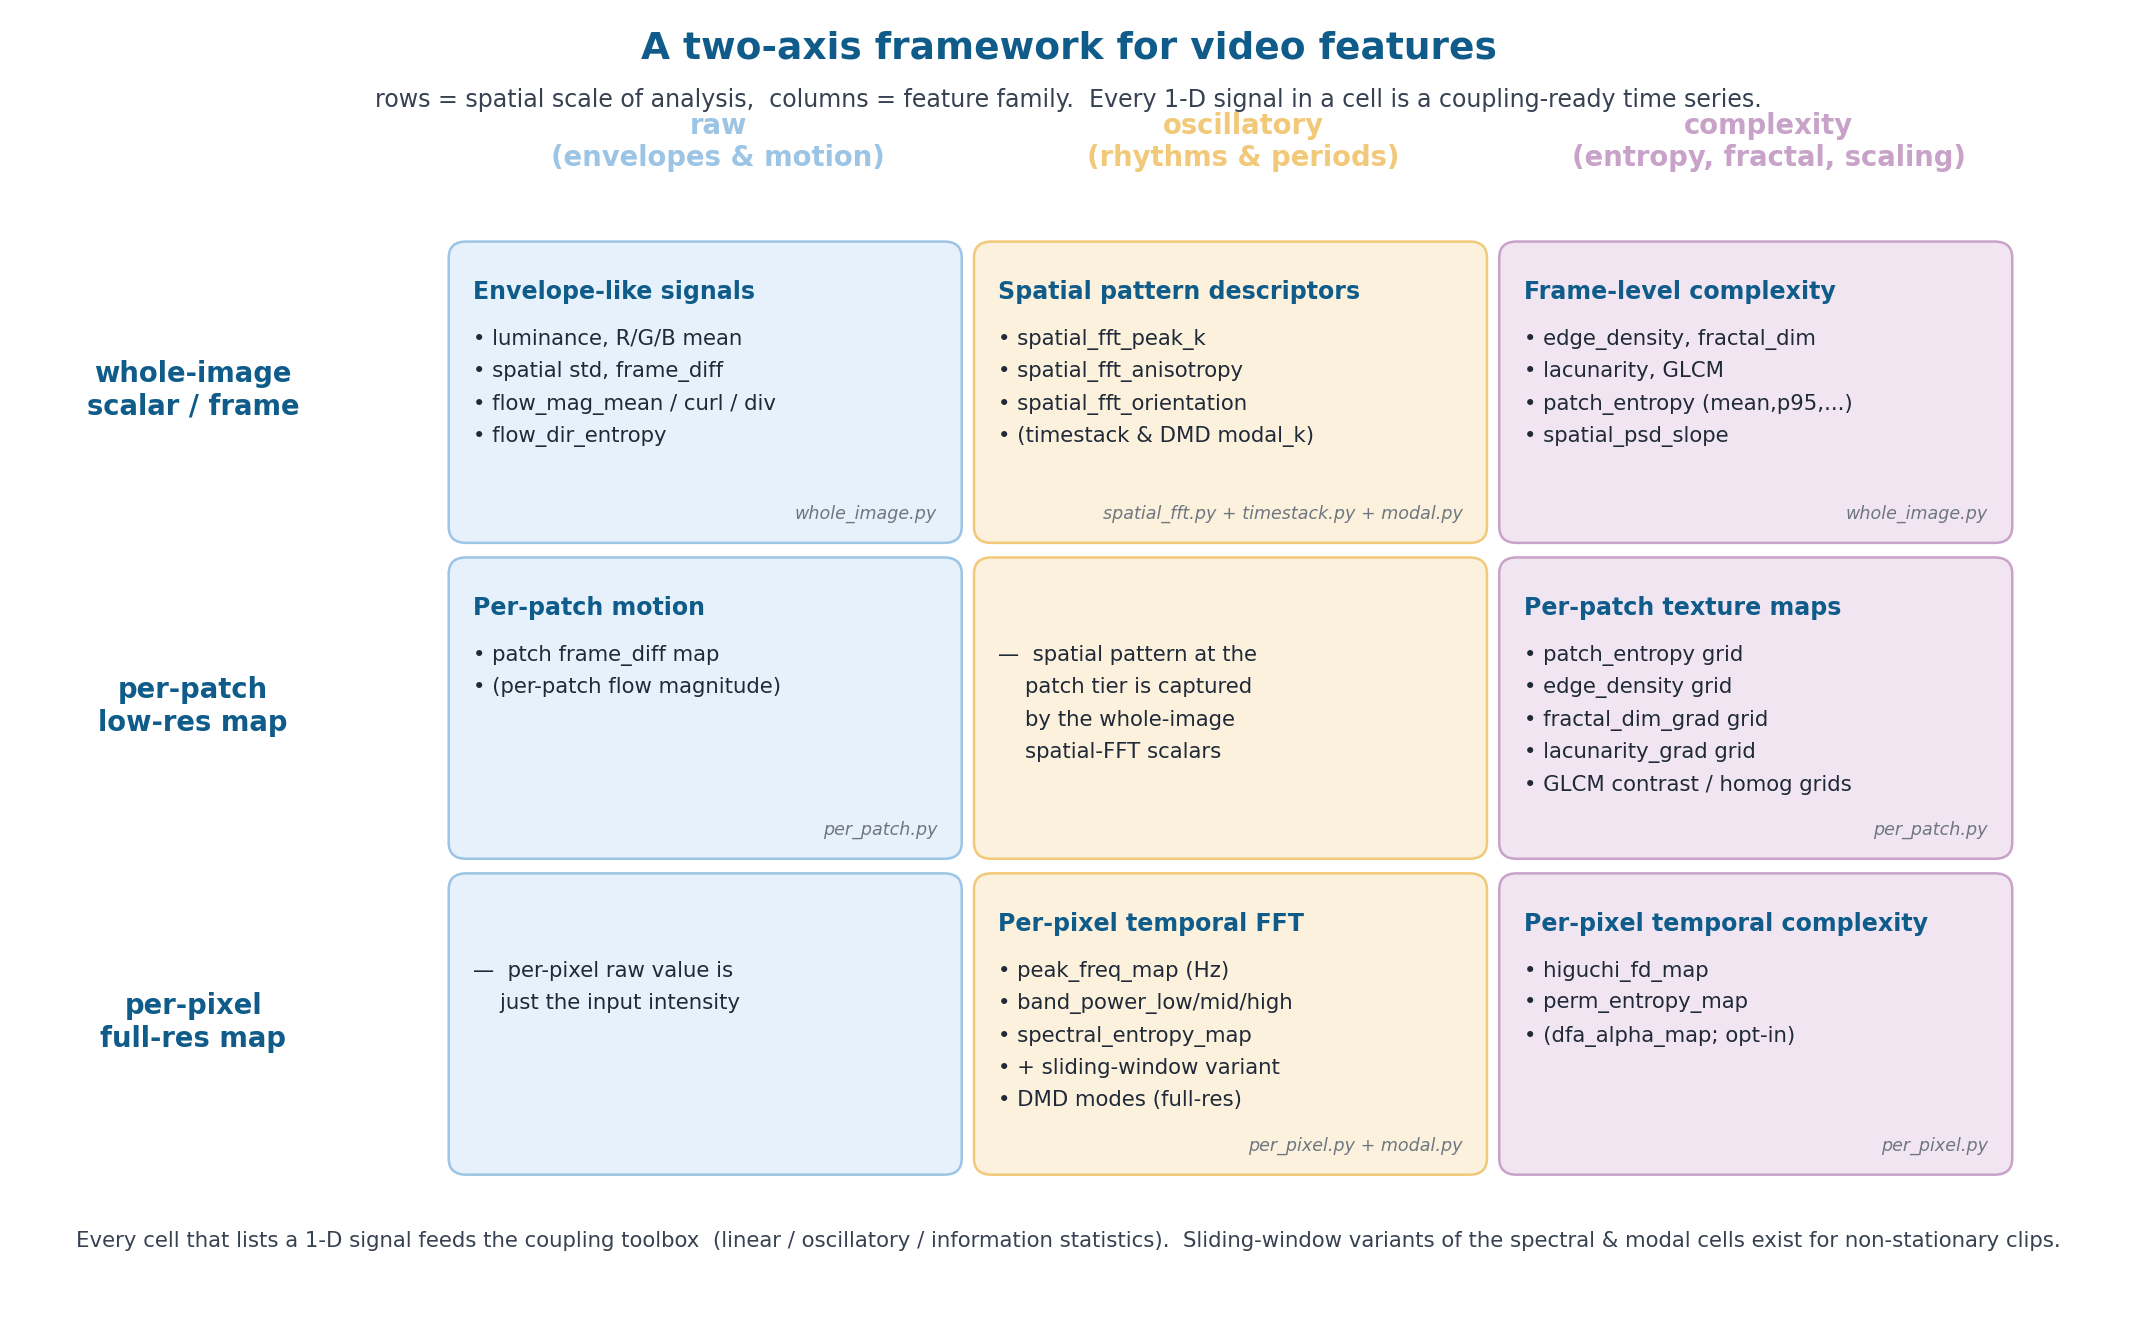
\includegraphics[width=\linewidth]{figures/framework.png}
  \caption{\textbf{Two axes.} \emph{Rows} are the spatial scale at
  which a measurement is made: one scalar per frame (top), a
  low-resolution patch grid (middle), or one number per pixel
  (bottom). \emph{Columns} are the family of question we ask of the
  scene: a \famraw{raw value}, an \famosc{oscillation rate}, or a
  \famcpl{complexity summary}. Annotations under each cell name the
  source file in \code{src/HNA/modalities/video/}, so the figure doubles
  as a code map.}
  \label{fig:framework}
\end{figure}

\paragraph{Spatial scale (rows).}
\begin{itemize}[leftmargin=1.5em,itemsep=0.2em]
  \item \emph{Whole-image} -- one scalar per frame.
  \item \emph{Per-patch} -- a coarse $\sim$$8\!\times\!8$ grid of tile
        scalars per frame, returned as both a low-resolution map
        (visualisation) and a per-frame spatial mean (coupling).
  \item \emph{Per-pixel} -- every pixel of a downscaled frame keeps
        its own time series; the output is one full-resolution 2-D map
        per quantity.
\end{itemize}

\paragraph{Feature family (columns).}
\begin{itemize}[leftmargin=1.5em,itemsep=0.2em]
  \item \famraw{Raw} -- instantaneous values: luminance, colour means,
        frame difference, optical-flow magnitude / curl / divergence.
        The natural pair for a physiological raw envelope.
  \item \famosc{Oscillatory} -- ``what frequency?''. Timestack peak,
        DMD modes, 2-D-FFT spatial wavenumber, per-pixel temporal
        peak. The natural pair for a physiological rhythm (HRV LF/HF
        peak, EEG alpha peak).
  \item \famcpl{Complexity} -- ``how irregular?''. Edge density,
        fractal dimension, lacunarity, GLCM, patch entropy, $1/f$
        slope. The natural pair for a complexity time series on the
        physiology side.
\end{itemize}

The empty corner (per-pixel \famraw{raw}) is just the input intensity
itself and not interesting as a feature. Every other cell is populated.

% =========================================================================
\section{Four sea states as running examples}\label{sec:clips}
% =========================================================================

\begin{figure}[ht]
  \centering
  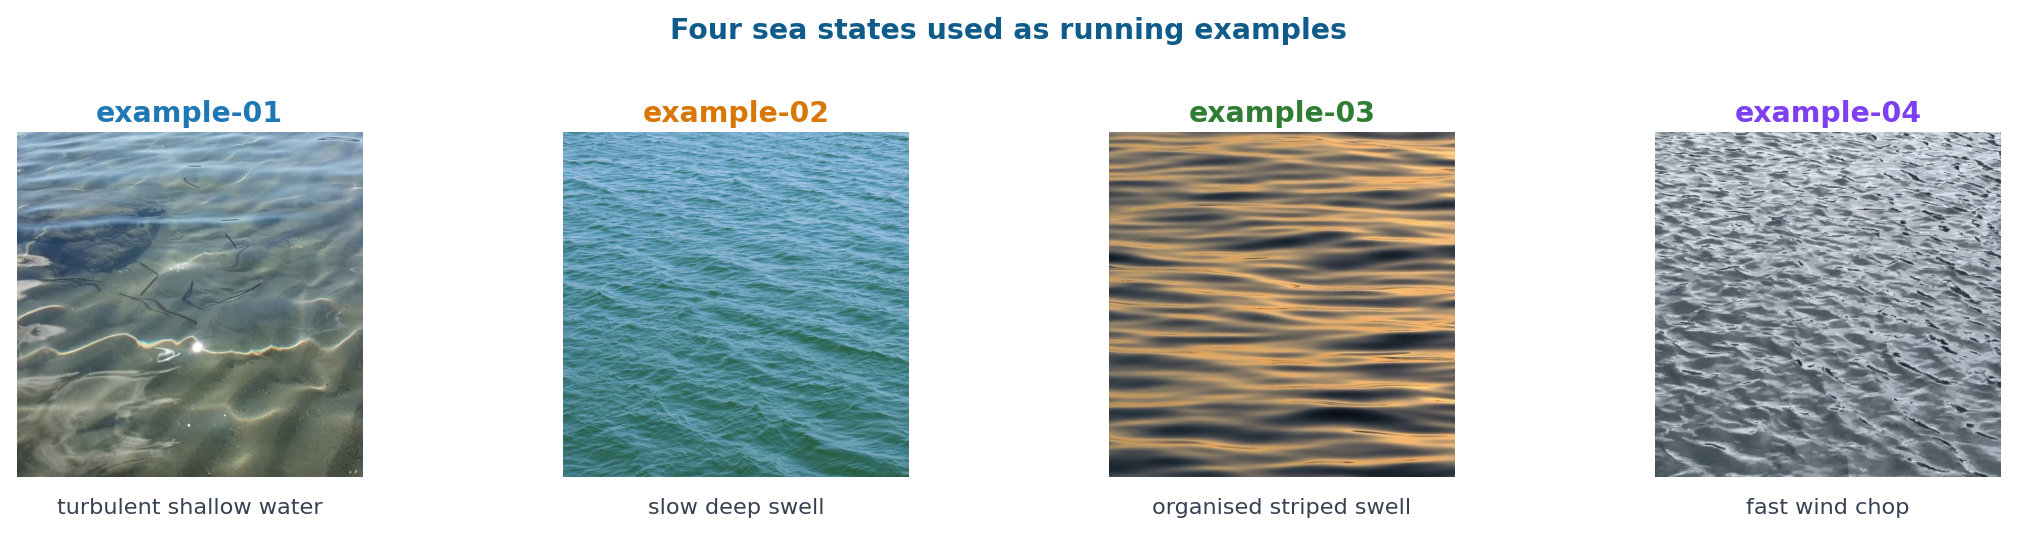
\includegraphics[width=\linewidth]{figures/v3_clips_overview.png}
  \caption{The four example clips used throughout this report. They
  bracket realistic conditions: a \textcolor{ex01}{turbulent shallow-
  water surf zone}; a \textcolor{ex02}{slow deep swell}; an
  \textcolor{ex03}{organised striped swell} dominated by horizontal
  crests; and \textcolor{ex04}{fast wind-driven chop}. Every figure
  below uses the same four clips and the same colour key.}
  \label{fig:clips}
\end{figure}

We picked four physically distinct clips that we expect to score
differently on most of the toolbox's metrics
(Fig.~\ref{fig:clips}). \textcolor{ex01}{ex-01} has the most motion
and the most local foam structure; \textcolor{ex02}{ex-02} is the
slowest and the most laminar; \textcolor{ex03}{ex-03} is the most
spatially regular (dominant horizontal stripes); \textcolor{ex04}{ex-04}
sits at the high-frequency end (fast wind chop, fine-scale texture).
Re-using the same four clips in every figure keeps the reader's eye
calibrated.

% =========================================================================
\section{Raw envelopes \& motion}\label{sec:raw}
% =========================================================================

The cheapest, most directly comparable family. A grayscale frame
collapses to seven scalars: mean luminance, per-channel R/G/B means,
spatial standard deviation, a $64$-bin Shannon entropy of intensity,
and the frame-to-frame absolute difference. Adding dense optical flow
gives mean magnitude, a 95th-percentile ``surge'' detector, mean
$|\mathrm{curl}|$ (rotational / turbulent content), mean divergence,
and the entropy of flow direction.

Fig.~\ref{fig:raw-motion} aligns three of these traces -- luminance,
flow magnitude, frame-difference -- across the four clips on a shared
$z$-score axis. The four sea states differ visibly in motion energy
and rhythm regularity: the swell of \textcolor{ex02}{ex-02} dominates
its luminance trace; \textcolor{ex01}{ex-01} oscillates broadly;
\textcolor{ex03}{ex-03}'s slow drift is striking against its
high-frequency frame-difference; \textcolor{ex04}{ex-04} packs every
luminance value into a tight, uniform high-frequency oscillation.

\begin{figure}[ht]
  \centering
  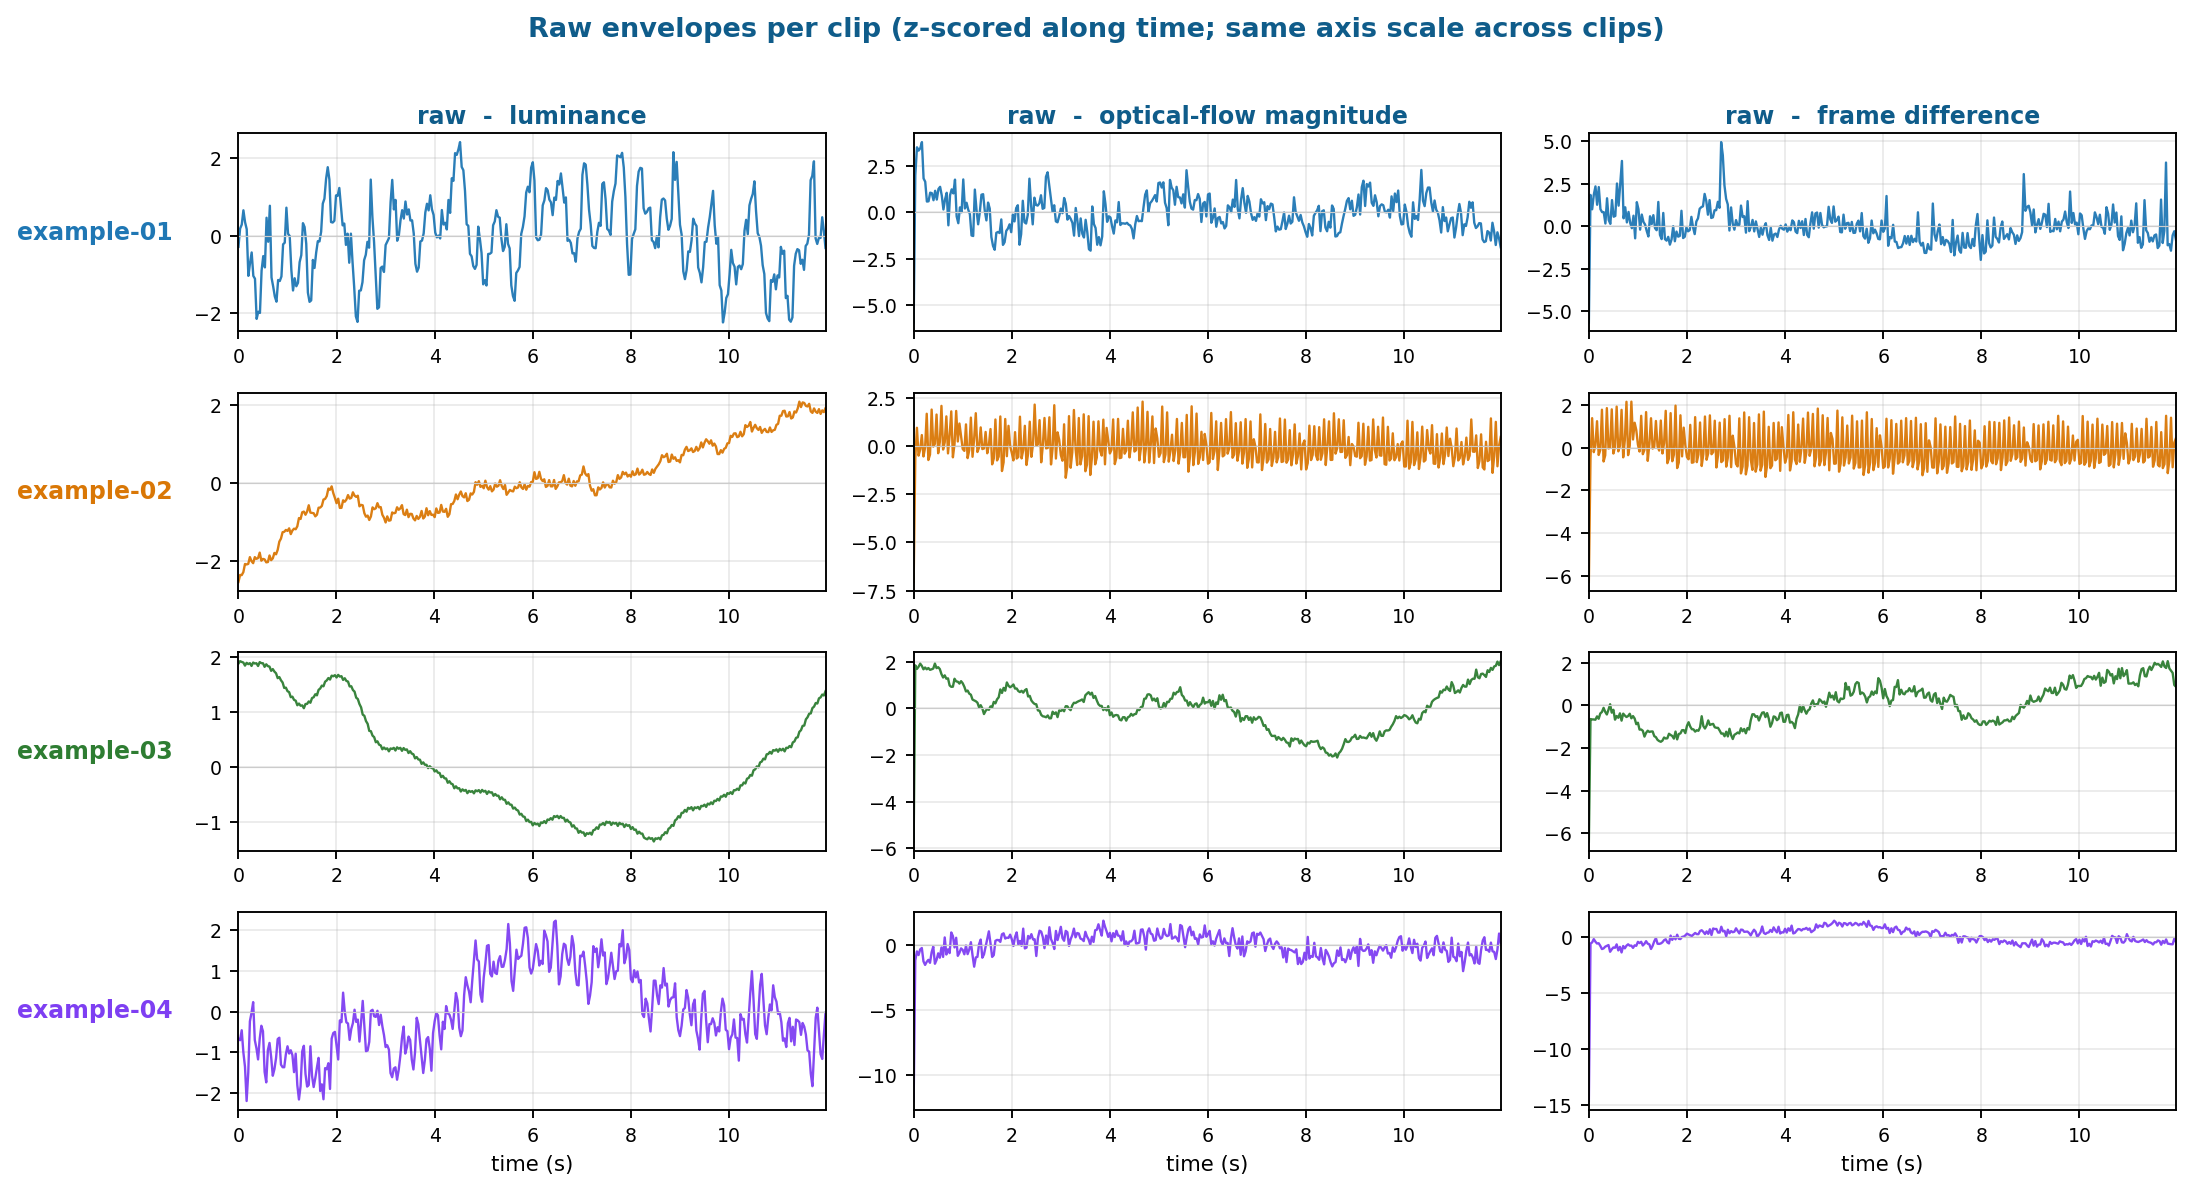
\includegraphics[width=\linewidth]{figures/v3_raw_motion.png}
  \caption{Three \famraw{raw} envelopes per clip ($z$-scored along
  time, same axis scale). Luminance, mean optical-flow magnitude,
  and per-frame absolute difference. These are the most direct visual
  analogue of an audio envelope; they pair naturally with respiration
  or EEG band-power on the coupling side.}
  \label{fig:raw-motion}
\end{figure}

\paragraph{Multi-scale flow.} Optical-flow magnitude at three
\emph{temporal strides} $\Delta t \in \{1, 3, 9\}$ frames isolates
ripple-scale motion ($\Delta t\!=\!1$), intermediate motion, and
quarter-swell motion ($\Delta t\!=\!9$ at $\sim\!30$~fps probes
$\sim\!0.3$~s). The same four scalars (mag, $|\mathrm{curl}|$, div,
direction entropy) are then computed on the full field, on its
Gaussian low-pass component (swell), and on the residual (turbulence),
giving $36$ frame-rate signals from one extractor
(Fig.~\ref{fig:multiscale-flow}).

\begin{figure}[ht]
  \centering
  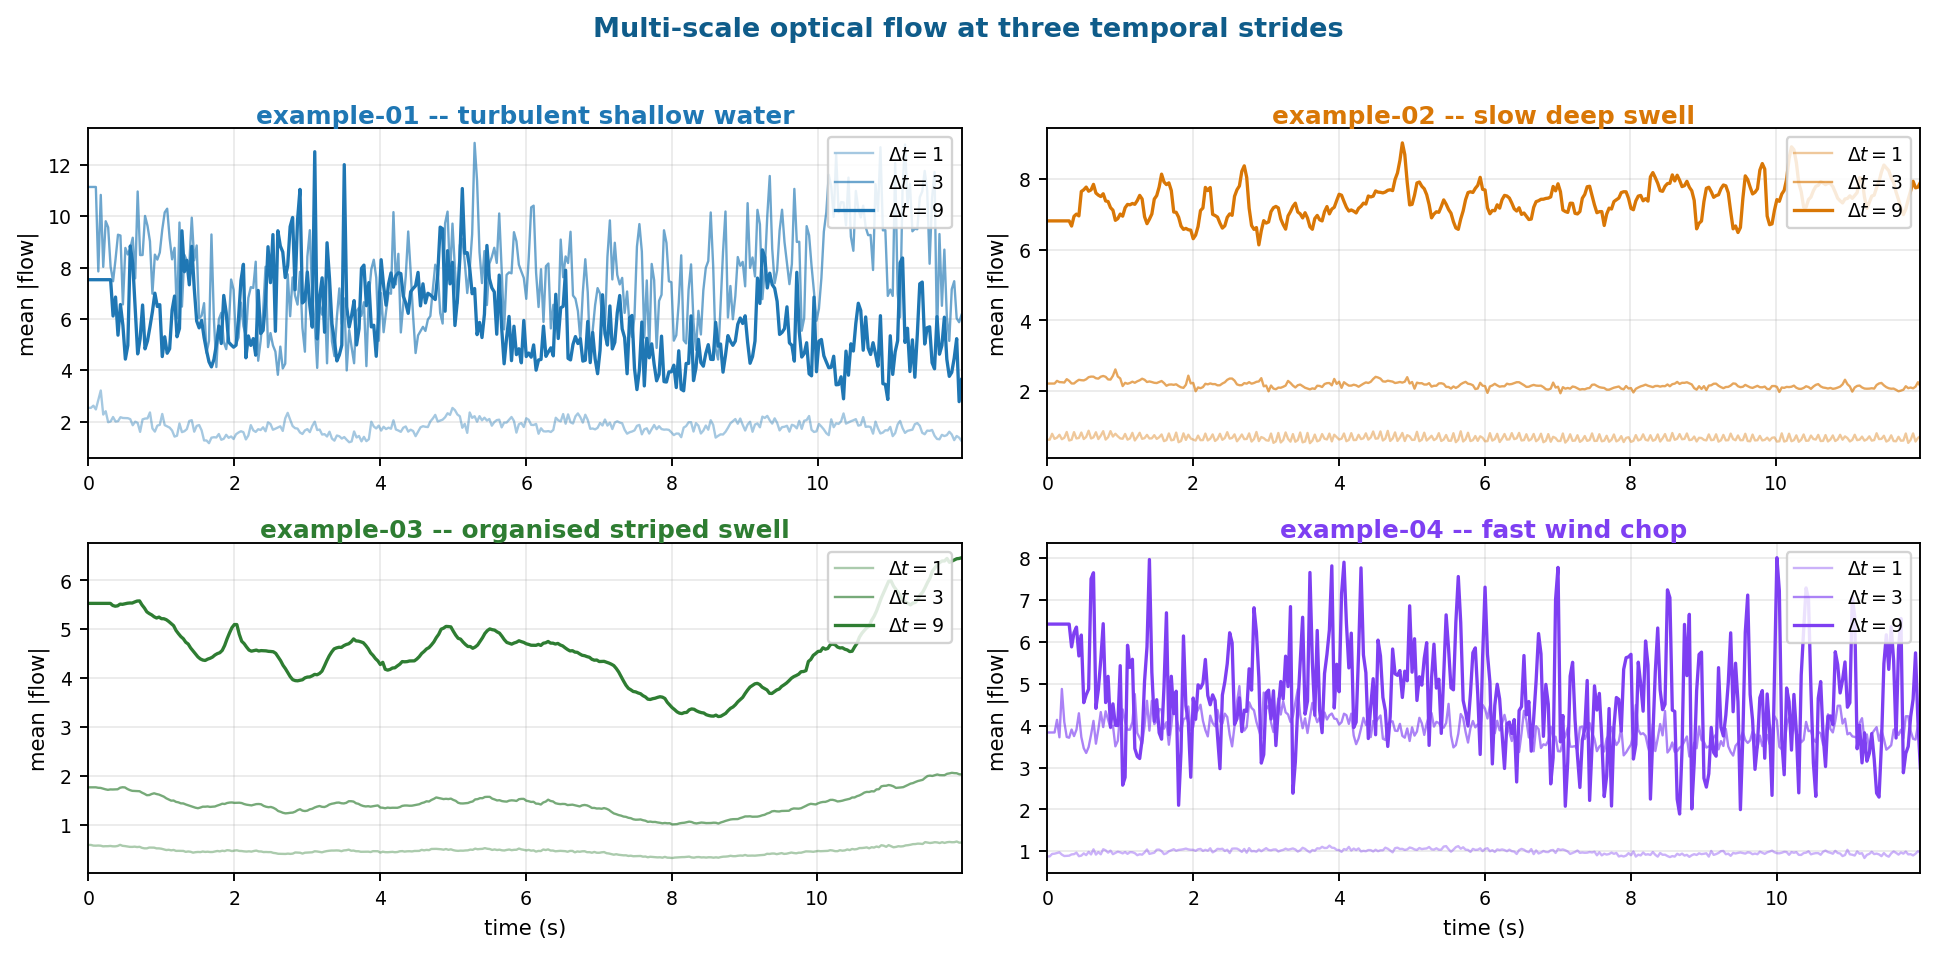
\includegraphics[width=\linewidth]{figures/v3_multiscale_flow.png}
  \caption{Multi-scale optical flow at the three strides, per clip.
  The longer the baseline, the more swell motion is integrated --
  hence the systematic offset between $\Delta t = 1$ and $\Delta t = 9$
  in every panel. \textcolor{ex02}{ex-02} (slow deep swell) shows the
  largest stride-9 mean: a slow but spatially coherent drift moves a
  lot of pixels per nine-frame jump.}
  \label{fig:multiscale-flow}
\end{figure}

% =========================================================================
\section{Oscillatory: rhythms and dominant periods}\label{sec:osc}
% =========================================================================

Three extractors live in this column at three different spatial
scales. Together they answer ``\emph{what is this clip's heartbeat?}''.

\subsection{Timestack -- whole-image scalar}

Borrowed from coastal remote sensing \citep{holman2007}: sample one
vertical column at every frame, average its rows, take the Welch PSD,
report the band-restricted argmax. That gives one scalar per clip
(the dominant wave frequency) plus the 1-D row-mean signal as a
coupling input. We measure $1.50$~Hz for \textcolor{ex01}{ex-01} and
$0.12$~Hz for the other three -- consistent with a fast-chopping
shallow-water surf zone vs.\ slower deep-water swells.

\subsection{Modal decomposition (DMD) -- per-pixel-resolution modes}
\label{sec:dmd}

DMD \citep{schmid2010,kutz2016,demo2018pydmd} fits one linear
evolution operator $X_{t+1} = A X_t$ to the (pixels~$\times$~time)
matrix and returns top-$k$ \emph{complex} eigenvalues, so each
spatio-temporal mode has a single frequency. (An SVD/POD baseline
pairs sin/cos at the same frequency: a single-component sea at
$f_p\!=\!0.125$~Hz produces four POD modes at
$\{0.125, 0.125, 0.250, 0.250\}$~Hz -- visually similar and
spectrally indistinguishable. DMD removes that redundancy.)

\begin{figure}[ht]
  \centering
  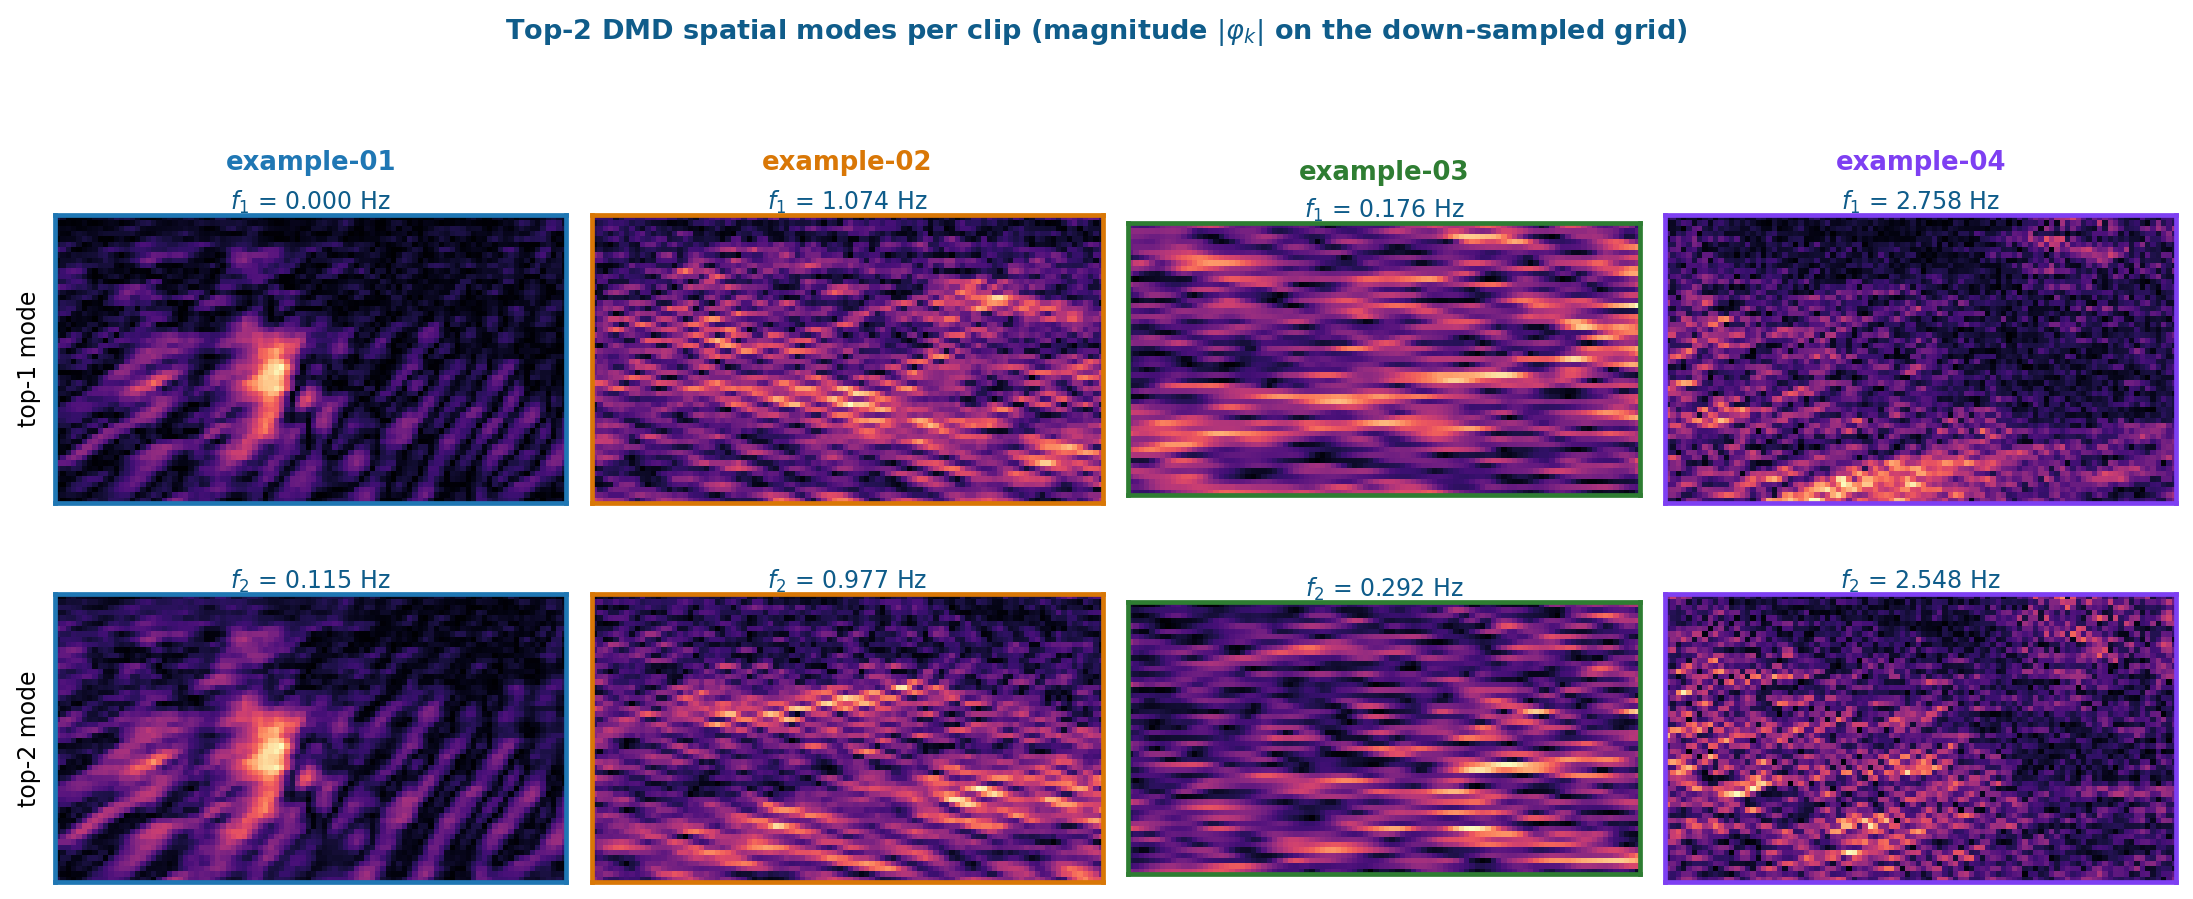
\includegraphics[width=\linewidth]{figures/v3_dmd_top_modes.png}
  \caption{Top-2 \famosc{DMD spatial modes} for each clip,
  $|\varphi_k|$ on the down-sampled grid. Frequencies
  $f_k = |\omega_k|/2\pi$ printed above each panel. \textbf{The
  modes are derived per clip}: each clip has its own decomposition,
  and the spatial patterns differ accordingly --
  \textcolor{ex01}{ex-01} concentrates energy in foreground foam,
  \textcolor{ex02}{ex-02} shows a smooth large-scale swell pattern,
  \textcolor{ex03}{ex-03} resolves the dominant horizontal stripe of
  the regular swell, \textcolor{ex04}{ex-04} is fine-scale turbulent
  texture at high frequency.}
  \label{fig:dmd}
\end{figure}

The frequencies ladder up cleanly across the four clips: ex-03 places
its top modes near $0.18$ -- $0.29$~Hz (a slow regular swell);
ex-02 puts both top modes around $1.0$~Hz; ex-01 has two distinct
modes at $0$~Hz (a stationary mean-removed component) and $0.12$~Hz;
ex-04 sits at $2.5$~Hz and above (Fig.~\ref{fig:dmd}). Each mode's
real-valued temporal coefficient is exposed as a 1-D signal in
\code{feats.signals} under the keys \code{modal\_1}, \code{modal\_2},
\dots.

\subsection{Per-pixel temporal FFT -- per-pixel maps}\label{sec:pixspec}

The most spatially detailed of the three: every pixel of a downscaled
copy keeps its own dominant frequency, its own spectral entropy, its
own band powers. The result is a small set of 2-D maps and two
clip-level scalars -- \code{sync\_index} (concentration of the mean
spectrum) and \code{coherence\_index} (spatial uniformity of peak
frequency). The maps themselves answer ``\emph{which part of the
frame is the swell, which part is the foam?}''
(Fig.~\ref{fig:pixspec}).

\begin{figure}[ht]
  \centering
  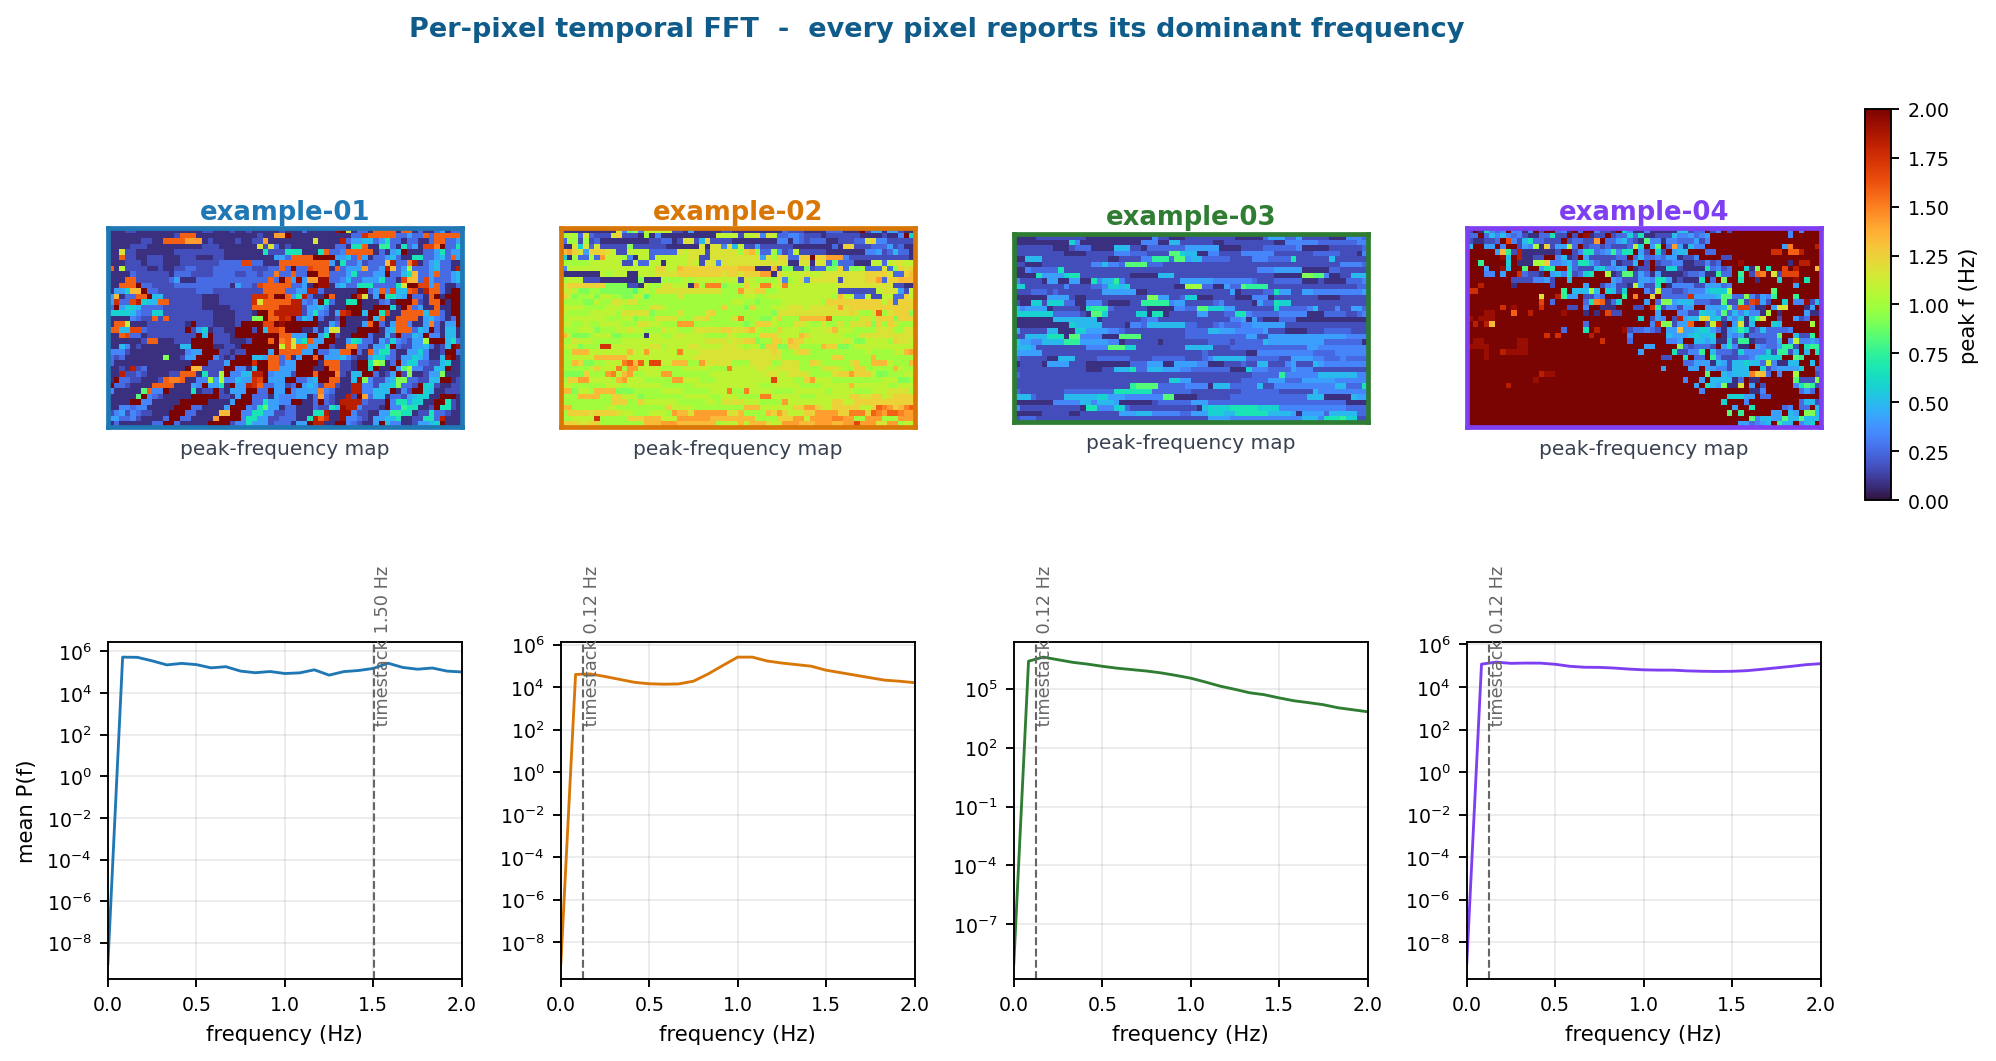
\includegraphics[width=\linewidth]{figures/v3_pixel_spectrum.png}
  \caption{Per-pixel temporal FFT. Top: peak-frequency map -- every
  pixel coloured by the frequency at which it oscillates the most.
  Bottom: mean spectrum across pixels, with the timestack peak marked
  for reference. Note the clean spatial structure on
  \textcolor{ex02}{ex-02} (a near-uniform $\sim\!1$~Hz pulse over the
  whole frame) versus the fragmented, foam-dominated map on
  \textcolor{ex01}{ex-01}; \textcolor{ex04}{ex-04} divides into
  high-frequency wind-chop (red) and slow background (blue).}
  \label{fig:pixspec}
\end{figure}

\subsection{Spatial pattern (2-D FFT)}\label{sec:spatial-fft}

A different kind of ``oscillatory'': not in time but in space. The
2-D Fourier transform of a single frame gives a peak radial
wavenumber (the dominant spatial period of foam / ripple texture), a
horizontal-vs-vertical anisotropy (positive when horizontal swell
crests dominate), and a weighted-mean orientation. In our four-clip
fingerprint (Fig.~\ref{fig:fingerprint}, oscillatory band) the
anisotropy peaks at $3.11$ on \textcolor{ex03}{ex-03} -- the only
clip with a tightly aligned striped swell -- and is positive on every
clip we sampled.

\subsection{Sliding-window variants for non-stationary clips}

Three of the cells above -- per-pixel FFT, DMD, and timestack PSD --
are by default \emph{single-window} estimators: they fit one model to
the whole clip. Whenever the clip is long enough that the dominant
frequency may drift (a swell building, the wind freshening), a single
window is too coarse. We expose sliding-window counterparts that
promote those summaries to 1-D signals at frame rate:
\code{extract\_pixel\_spectrum\_windowed},
\code{extract\_modal\_windowed}, \code{extract\_timestack\_windowed}.
They share the parameters \code{windowed\_win\_sec} (default $4$~s)
and \code{windowed\_step\_sec} (default $0.5$~s); per-window values
are linearly interpolated onto the frame grid so they line up with
everything else.

% =========================================================================
\section{Complexity: roughness, clumpiness, irregularity}\label{sec:cplx}
% =========================================================================

The third column collects every measure that asks ``\emph{how complex
is this?}'' rather than ``\emph{what value, what frequency?}''.

\paragraph{Frame-level scalars.} Edge density (Canny), the
radial-PSD slope (parallel to the EEG aperiodic $1/f$ exponent),
box-counting fractal dimensions on two binarisations of the frame
(Canny edges and gradient-magnitude), Plotnick / Allgood lacunarity
on those same binarisations, GLCM contrast / homogeneity, and the
patch-Shannon-entropy mean. $D$ (fractal dimension) and $\Lambda$
(lacunarity) are \emph{complementary}: $D$ is nearly identical
across the four sea states (they all sit near $2.05$), but $\Lambda$
on the gradient image splits them strongly
(Fig.~\ref{fig:complexity}).

\begin{figure}[ht]
  \centering
  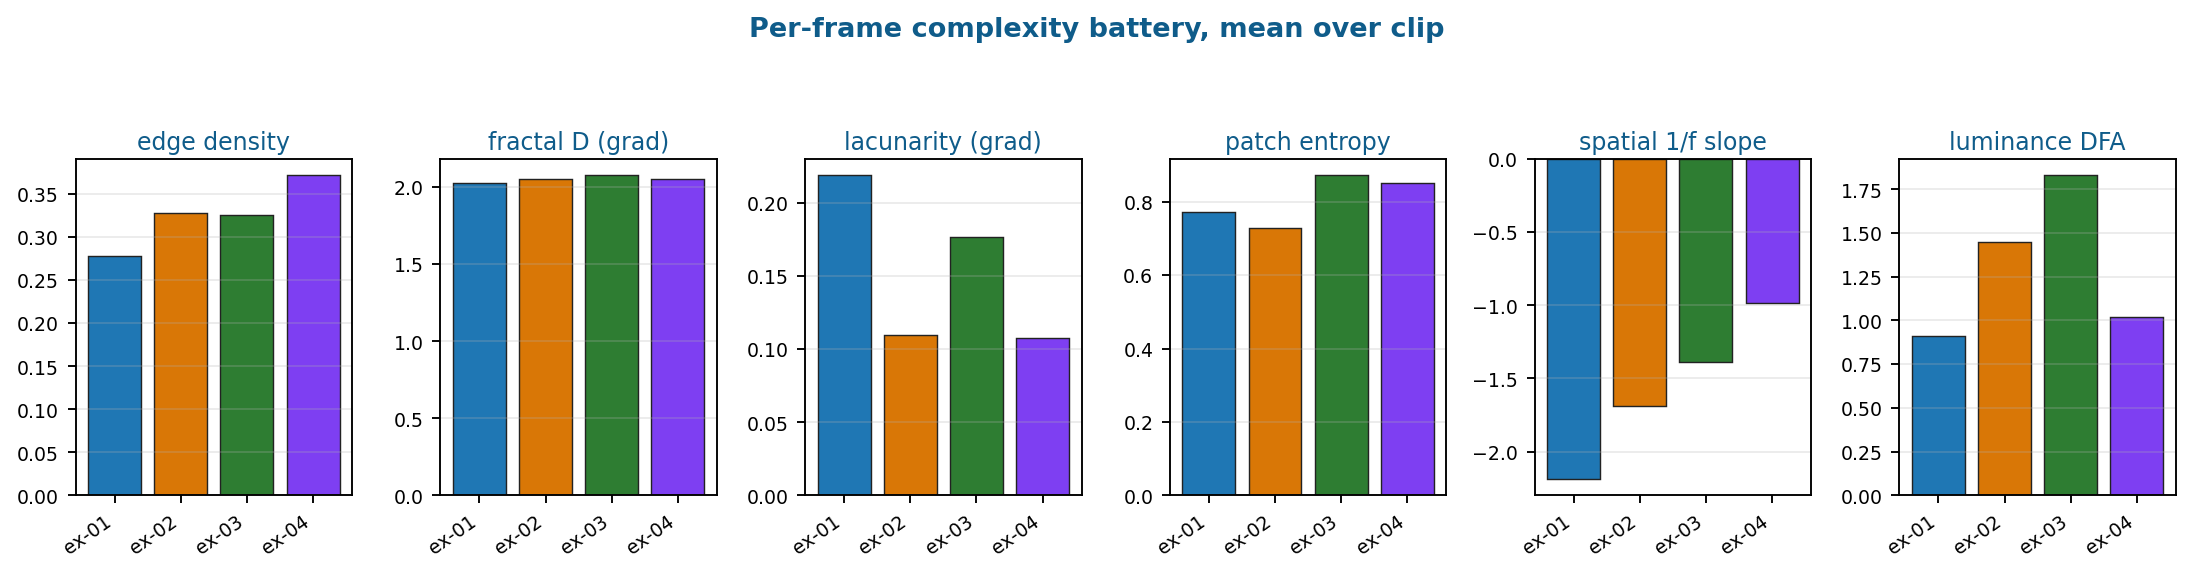
\includegraphics[width=\linewidth]{figures/v3_complexity.png}
  \caption{Six \famcpl{complexity} measures, mean over each clip.
  Edge density and patch entropy push \textcolor{ex04}{ex-04}
  highest (foam everywhere, broad intensity histogram in every
  patch); fractal dimension is essentially flat across clips, but
  lacunarity is not; and the spatial $1/f$ slope is steepest for
  \textcolor{ex01}{ex-01} (heavy low-spatial-frequency content from
  the foreground swell). Luminance DFA, by contrast, is highest for
  \textcolor{ex03}{ex-03}, where the slow regular swell makes the
  luminance envelope look long-range correlated.}
  \label{fig:complexity}
\end{figure}

\paragraph{Per-patch maps (\code{extract\_spatial\_field}).}
The same frame-level descriptors recomputed inside every patch of an
$\sim\!8\!\times\!8$ grid. Each call returns both a $(G_y, G_x, T)$
stack of patch maps for visualisation and the per-frame spatial mean
of each map as a 1-D signal (suffix \code{field\_*}). This fills the
per-patch row of the framework -- previously sparse -- and surfaces
the within-frame heterogeneity that the clip-level mean throws away.

\paragraph{Per-pixel temporal complexity
(\code{extract\_pixel\_complexity}).}
The deepest spatial reduction: at every pixel of a downscaled copy,
run a Higuchi fractal dimension and a permutation entropy (and
optionally DFA) on the luminance time series. The output is a
full-resolution 2-D map per measure -- ``\emph{where on the frame is
the temporal behaviour most complex?}''. Opt-in because it is the
toolbox's most expensive operation.

\paragraph{The 15-measure summary, applied to every 1-D signal.}
Independently of the maps, every 1-D signal in \code{feats.signals}
is also summarised by 15 nonlinear-dynamics measures via
\code{complexity\_summary}: five entropies, three fractal dimensions,
Hjorth mobility / complexity, DFA, Hurst, Lempel--Ziv, multiscale
entropy area, and the $1/f$ slope. The reason to repeat them on
every signal is that ``complexity'' is multifaceted: two signals can
match on entropy and disagree on fractal dimension. Reporting all
15 and letting the downstream analysis pick keeps options open. The
same library implementations (\code{antropy}, \code{neurokit2}) are
used on the EEG/HRV side, so cross-modal complexity comparisons are
apples-to-apples.

% =========================================================================
\section{Cross-clip fingerprint, organised by family}\label{sec:fingerprint}
% =========================================================================

\begin{figure}[ht]
  \centering
  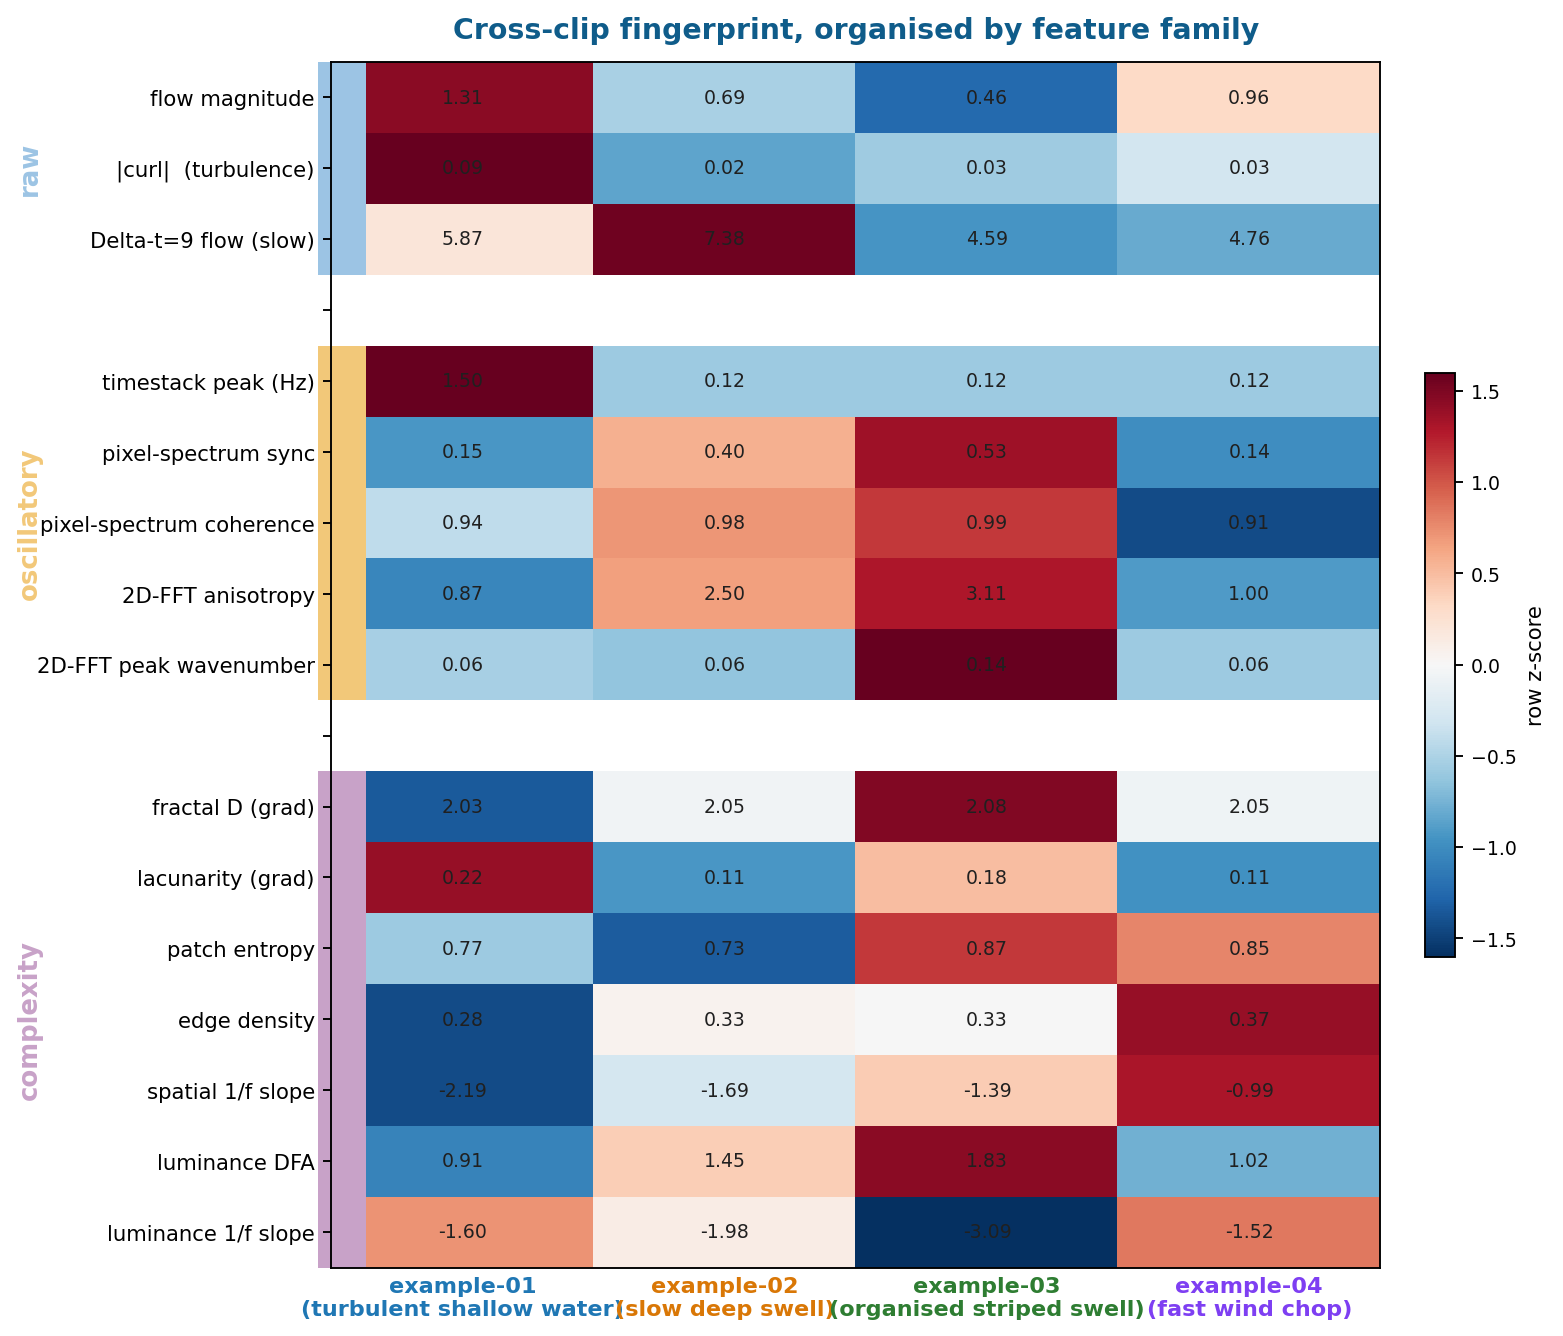
\includegraphics[width=0.92\linewidth]{figures/v3_fingerprint.png}
  \caption{Cross-clip fingerprint with rows grouped by feature family
  (left side stripes). Each cell text is the raw metric; the colour
  is the row $z$-score across the four clips, so within each row the
  most extreme cell is the most informative. The blocks make a
  visible structural point: a clip's signature is not a single
  number but a \emph{pattern of agreements and disagreements} across
  families. \textcolor{ex01}{ex-01} is the only clip where the
  \famosc{timestack peak} is dominant; \textcolor{ex03}{ex-03} owns
  almost every \famosc{oscillatory} cell (high pixel-spectrum sync,
  high coherence, high 2-D-FFT anisotropy); \textcolor{ex04}{ex-04}
  wins the \famcpl{complexity} bands on edge density and gradient
  fractal dimension.}
  \label{fig:fingerprint}
\end{figure}

The reason this figure exists is exactly the point we keep coming
back to: \emph{no single video metric is a perfect summary, and
that is the point}. Each metric is sensitive to a different physical
facet of the scene; the union is the clip's signature. Reading
horizontally tells you which clip wins on a given metric; reading
vertically tells you the clip's identity. The family-grouped layout
makes the second reading much easier than a flat heatmap because the
question is no longer ``\emph{is this row important?}'' but
``\emph{which family is most informative for this clip?}''.

% =========================================================================
\section{From features to coupling}\label{sec:coupling}
% =========================================================================

Every signal in \code{feats.signals} is a 1-D \code{np.ndarray}
sampled at $f_s = \code{feats.fs}$ and is therefore an immediate
input to \code{HNA.modules.coupling}. The coupling toolbox itself
organises into three families that mirror the feature columns
(Table~\ref{tab:coupling}).

\begin{table}[ht]
\centering
\small
\renewcommand{\arraystretch}{1.18}
\setlength{\tabcolsep}{8pt}
\begin{tabularx}{\linewidth}{l X X}
\toprule
\textbf{Coupling family} & \textbf{Statistics} &
   \textbf{Pair naturally with} \\
\midrule
\textbf{Linear}  & windowed cross-correlation,
                   magnitude-squared coherence,
                   peak $r$ + lag &
                   \famraw{raw} envelopes (\code{luminance},
                   \code{flow\_mag\_mean}, \code{frame\_diff})
                   vs.\ respiration / EEG band power. \\
\textbf{Oscillatory} & phase-locking value (PLV),
                       weighted phase-lag index (wPLI) &
                       \famosc{oscillatory} signals
                       (\code{modal\_1},
                        \code{timestack\_w\_peak\_freq\_hz},
                        \code{pixspec\_w\_peak\_freq\_median})
                       vs.\ HRV LF/HF peak, EEG alpha-peak
                       frequency. \\
\textbf{Information} & mutual information,
                       transfer entropy &
                       \famcpl{complexity}-paired signals
                       (\code{wc\_flow\_mag\_mean\_\_higuchi\_fd},
                        \code{wc\_patch\_entropy\_\_perm\_entropy})
                       vs.\ rolling Higuchi FD or permutation
                       entropy on EEG / HRV. \\
\bottomrule
\end{tabularx}
\caption{Three coupling families on the physiology side, mirrored to
the three feature families on the video side. The right column shows
pairings where ``same family on both sides'' yields the most
interpretable estimate.}
\label{tab:coupling}
\end{table}

\begin{lstlisting}
from HNA.modalities.video import quantify_video
from HNA.modules.coupling import (
    windowed_xcorr, band_coherence,        # linear
    plv_phase_sync, wpli_phase_sync,        # oscillatory
)

feats = quantify_video("video_examples/example-01.mp4",
                       include_pixel_spectrum_windowed=True,
                       include_modal_windowed=True,
                       include_timestack_windowed=True,
                       include_spatial_field=True,
                       include_pixel_complexity=True)

# linear: video luminance vs. respiration envelope
xc  = windowed_xcorr(feats.signals["luminance"], respiration,
                     fs=feats.fs, win_sec=180, step_sec=10,
                     max_lag_sec=30)
# oscillatory: instantaneous wave frequency vs. EEG alpha-peak
plv = plv_phase_sync(feats.signals["timestack_w_peak_freq_hz"],
                     eeg_alpha_peak_f, fs=feats.fs)
\end{lstlisting}

% =========================================================================
\section{Practical recipe}\label{sec:recipe}
% =========================================================================

\paragraph{Default call.}
\begin{lstlisting}
from HNA.modalities.video import quantify_video
feats = quantify_video("path/to/clip.mp4")
\end{lstlisting}
That gets you envelopes, single-scale optical flow, frame-level
spatial complexity, 2-D-FFT scalars, the timestack, top-4 DMD modes,
and the 15-measure complexity summary on every signal. About
$5$~seconds for a 20-second HD clip on CPU.

\paragraph{Add what you need.} The opt-in flags map one-to-one to
cells of Fig.~\ref{fig:framework}:
\begin{itemize}[leftmargin=1.5em,itemsep=0.2em]
  \item \code{include\_spatial\_field=True} -- per-patch maps + means
        (per-patch row, all three feature columns).
  \item \code{include\_pixel\_spectrum=True} -- per-pixel temporal
        FFT maps (per-pixel \famosc{oscillatory}).
  \item \code{include\_pixel\_complexity=True} -- per-pixel temporal
        complexity maps (per-pixel \famcpl{complexity}; opt-in
        because it is the most expensive operation).
  \item \code{include\_pixel\_spectrum\_windowed=True} \quad /
        \quad \code{include\_modal\_windowed=True} \quad /
        \quad \code{include\_timestack\_windowed=True} -- the
        sliding-window counterparts, for non-stationary clips.
  \item \code{include\_windowed\_complexity=True} -- promote any 1-D
        signal's complexity to a 1-D series.
\end{itemize}

\paragraph{File layout under \code{src/HNA/modalities/video/}.} The
sub-package mirrors Fig.~\ref{fig:framework} cell by cell:

\begin{lstlisting}
src/HNA/modalities/video/
  _common.py             # frame I/O, probe, iter_frames, _stack_video
  whole_image.py         # global signals, optical flow, spatial complexity
  spatial_fft.py         # per-frame 2-D-FFT scalars
  per_patch.py           # extract_spatial_field
  per_pixel.py           # pixel_spectrum + extract_pixel_complexity
  modal.py               # DMD (global + windowed)
  timestack.py           # timestack (global + windowed)
  temporal_complexity.py # complexity_summary, windowed_complexity
  pipeline.py            # quantify_video
\end{lstlisting}

The public API is exposed at the top level of the sub-package:
\code{from HNA.modalities.video import quantify\_video, extract\_<name>, ...}.

\paragraph{Defaults worth knowing.}
The whole pipeline runs on a $192$-px-on-the-long-axis grayscale copy
of the video; the modal decomposition uses a $96$-px copy; per-pixel
complexity uses an even smaller $48$-px copy by default. Patch size
is $24$~px ($\sim\!8\!\times\!8$ grid). Sliding-window defaults are
$W = 4$~s, $h = 0.5$~s for the spectral / modal / timestack family
and $W = 2$~s, $h = 0.25$~s for the complexity family. The full
hyperparameter list is documented inline in each extractor's
docstring.

% =========================================================================
\section*{Reproducibility}
\addcontentsline{toc}{section}{Reproducibility}
% =========================================================================

\begin{lstlisting}
# 1. Install the package with the video extras (opencv-python, scipy,
#    antropy, neurokit2, pydmd). antropy / neurokit2 / pydmd gracefully
#    degrade to NaN where unavailable; opencv-python is required.
pip install -e .[video]

# 2. Quantify a single clip
python -c "from HNA.modalities.video import quantify_video; \
           f = quantify_video('video_examples/example-01.mp4'); \
           print(len(f.signals), 'signals at', f.fs, 'Hz')"

# 3. Re-render the report figures
python scripts/figures/video_v3/framework.py   # framework.png
python scripts/figures/video_v3/all_figures.py         # v3_*.png

# 4. Compile the report
tectonic report/main_v3.tex
\end{lstlisting}

\end{document}
